\documentclass[12pt, letterpaper]{article}

\usepackage[utf8]{inputenc}
\usepackage[T1]{fontenc}
\usepackage[margin=1in]{geometry}
\usepackage{amsmath}
\usepackage{booktabs}
\usepackage{enumitem}
\usepackage[hidelinks]{hyperref}
\usepackage{float}
\usepackage{graphicx}
\usepackage{tikz}
\usetikzlibrary{shapes, arrows.meta, positioning, calc, fit, backgrounds}

\title{\textbf{Project Proposal: FPGA-Based MLP Accelerator for Handwritten Digit Recognition}\\[6pt]}
\date{}

\begin{document}

\maketitle

\begin{center}
\textbf{Course:} CMPE 240 Sec 01: Advanced Computer Design\\[10pt]
\textbf{Platform:} Digilent Zybo Z7-10 (Zynq-7010 SoC)\\[10pt]
\textbf{Toolchain:} Xilinx Vivado Design Suite\\[16pt]
\textbf{Project Group 1:}\\[6pt]
\begin{tabular}{cccc}
\toprule
\textbf{\#} & \textbf{Name} & \textbf{Student ID} \\
\midrule
1 & Simul Barua & 018315661 \\[6pt]
2 & Sriram Sridhar & 016661411 \\[6pt]
3 & Manisha Varthamanan & 020095920 \\[6pt]
4 & Urmi Shah & 019107595 \\[6pt]
5 & Anusha Subramanian & 014122459 \\[6pt]
6 & Nkono Andrew Mwase & 014224548 \\
\bottomrule
\end{tabular}
\end{center}

\bigskip\bigskip
`'
% ── 1. Introduction ────────────────────────────────────────────────────────────
\newpage
\section{Introduction}

For this project, we plan to design and implement a hardware accelerator for a
Multi-Layer Perceptron (MLP) on the Digilent Zybo Z7-10 board. The goal is to
classify handwritten digits (0--9) using the Programmable Logic (PL) fabric of
the Zynq-7010 SoC. This proposal explains why we chose the MLP model, describes
the dataset and training process, and presents our hardware design and implementation
plan.

The project is split into two phases. In Phase 1, we will train a small MLP in PyTorch
and quantize the learned weights to 8-bit integers, producing coefficient files
ready for FPGA deployment. In Phase 2, we will implement the MLP as a custom RTL accelerator
in the PL of the Zybo Z7-10. The Processing System (PS) will handle image
transfer and control, while the PL will run the MLP inference using the weights from Phase 1.\\[4pt]

\textbf{Key objectives:}
\begin{enumerate}
    \item Train a small MLP achieving $\geq 95\%$ accuracy on the MNIST test set.
    \item Quantize weights to 8-bit fixed-point to fit within the Z7-10's BRAM.
    \item Implement the MLP as an RTL datapath interfaced to the PS via AXI.
    \item Verify correct end-to-end inference on the hardware platform.
\end{enumerate}

% ══════════════════════════════════════════════════════════════════════════════
\section{Phase 1: Software Pipeline}
% ══════════════════════════════════════════════════════════════════════════════

Phase 1 covers everything that runs on a host PC: downloading and preparing
the MNIST dataset, training the MLP, quantizing its weights, and exporting the
coefficient files that Phase 2 will load into BRAM.\\[4pt]

\textbf{Phase 1 deliverables:}
\begin{enumerate}
    \item Download, pre-process, and validate the MNIST dataset pipeline.
    \item Train a floating-point MLP achieving $\geq 97\%$ test accuracy.
    \item Apply symmetric post-training INT8 quantization; verify $\geq 95\%$
          accuracy is retained.
    \item Export quantized weights, biases, and scale factors as \texttt{.coe}
          files ready for Vivado BRAM initialization.
\end{enumerate}

% ── 2.1 Model Selection ───────────────────────────────────────────────────────
\subsection{Model Selection}

The Zybo Z7-10 is a low-cost development board built around the Zynq-7010, which
is one of the smaller devices in the Zynq-7000 family. Its PL fabric is limited
to 17,600 LUTs, 80 DSP slices, and 60 BRAM blocks. Table~\ref{tab:zynq7010_resources} summarizes
the main PL resources available on the device and explains how each one affects the
hardware design choice.

\begin{table}[H]
\centering
\caption{Zynq-7010 PL Resource Summary}
\label{tab:zynq7010_resources}
\begin{tabular}{llp{8.5cm}}
\toprule
\textbf{Resource} & \textbf{Available} & \textbf{Design Implication} \\
\midrule
LUTs               & 17,600 & Limits combinational logic and makes large models difficult to implement \\
Flip-Flops         & 35,200 & Adequate for pipeline registers and FSM control \\
Block RAM (36\,Kb) & 60     & Approximately 270 KB in total; limits how many weights can be stored on-chip \\
DSP48E1            & 80     & Constrains parallel multiply-accumulate (MAC) units \\
\bottomrule
\end{tabular}
\end{table}

Given these constraints, we propose using a Multi-Layer Perceptron (MLP) instead of
a Convolutional Neural Network (CNN) for digit classification. Even a small CNN like LeNet-5 needs hundreds of thousands of parameters
and deeper MAC pipelines that exceed the Z7-10's DSP and BRAM budget. An MLP achieves sufficient accuracy
on MNIST (97\%--98\%), fits in BRAM after quantization, and has a simple structure that is easier to
implement in hardware.

% ── 2.2 MLP Architecture ──────────────────────────────────────────────────────
\subsection{MLP Architecture}

The selected MLP takes a flattened MNIST image as input, uses two hidden layers, and produces a 10-class output.
Table~\ref{tab:mlp_layers} summarizes its layer configuration.

\begin{table}[H]
\centering
\caption{MLP Layer Configuration}
\label{tab:mlp_layers}
\begin{tabular}{lcccc}
\toprule
\textbf{Layer} & \textbf{Input} & \textbf{Output} & \textbf{Activation} & \textbf{Parameters} \\
\midrule
FC1 (Hidden 1) & 784 & 64 & ReLU   & 50,240 \\
FC2 (Hidden 2) & 64  & 32 & ReLU   & 2,080  \\
FC3 (Output)   & 32  & 10 & Argmax & 330    \\
\midrule
\multicolumn{4}{l}{\textbf{Total Parameters}} & \textbf{52,650} \\
\bottomrule
\end{tabular}
\end{table}

Figure~\ref{fig:mlp} shows the overall structure of the MLP architecture.

\begin{figure}[H]
\centering
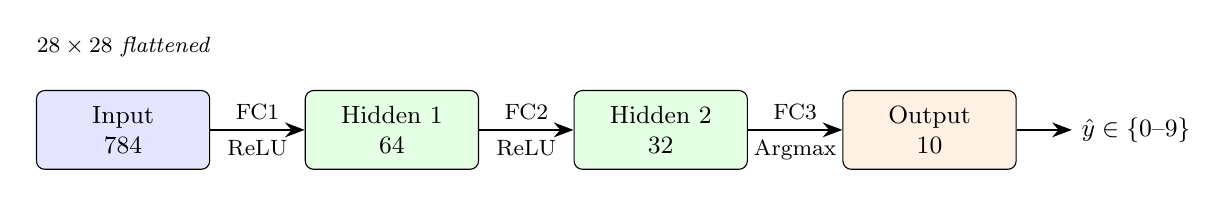
\begin{tikzpicture}[
    box/.style={draw, rounded corners=3pt, minimum height=1cm, align=center,
                font=\small, minimum width=2.2cm},
    arrow/.style={-{Stealth[length=2.5mm]}, thick},
    lbl/.style={font=\footnotesize, align=center},
]
\node[box, fill=blue!10]  (inp) {Input\\784};
\node[box, fill=green!10, right=1.2cm of inp] (h1)  {Hidden 1\\64};
\node[box, fill=green!10, right=1.2cm of h1]  (h2)  {Hidden 2\\32};
\node[box, fill=orange!10, right=1.2cm of h2] (out) {Output\\10};

\draw[arrow] (inp) -- node[above,lbl]{FC1} node[below,lbl]{ReLU} (h1);
\draw[arrow] (h1)  -- node[above,lbl]{FC2} node[below,lbl]{ReLU} (h2);
\draw[arrow] (h2)  -- node[above,lbl]{FC3} node[below,lbl]{Argmax} (out);

\node[above=0.3cm of inp, font=\footnotesize\itshape] {$28\times28$ flattened};
\node[right=0.7cm of out, font=\small] (mout) {$\hat{y}\in\{0\text{--}9\}$};
\draw[arrow] (out) -- (mout);
\end{tikzpicture}
\caption{MLP architecture: 784-input, two hidden layers (64 and 32 neurons), 10-class output.}
\label{fig:mlp}
\end{figure}

\textbf{784 inputs:} Each MNIST image is a $28\times28$ grayscale image. After flattening in row-major order, it becomes a 784-element vector that matches the input order used by the MLP.

\textbf{Two hidden layers (64 to 32):} Two hidden layers give the model enough capacity for handwritten digit recognition without making the hardware too large. The gradual reduction in size keeps the total parameter count low while still allowing the model to learn useful digit features.

\textbf{ReLU activations:} ReLU helps training and is simple to implement in hardware. On the FPGA, it only requires a comparison with zero.

\textbf{Argmax instead of Softmax:} Argmax gives the predicted class index, while Softmax gives probability scores. We only need the predicted class index for classification. Softmax requires exponentiation and division, which are expensive in fixed-point hardware. In contrast, Argmax only needs a simple comparator tree over the 10 outputs.

After 8-bit quantization, the 52,650 parameters require about 51.4\,KB of storage, which fits within the available BRAM of the Zynq-7010.

% ── 2.3 Pipeline Overview ─────────────────────────────────────────────────────
\subsection{Pipeline Overview}

Figure~\ref{fig:pipeline} shows the four stages of the Phase 1 software pipeline. All steps will run on the host PC; no FPGA hardware is needed for this phase. First, we will download and pre-process the MNIST dataset. Next, we will train and evaluate the floating-point MLP. After that, we will quantize the trained model to INT8 and verify that accuracy is retained. Finally, we will export the quantized weights and biases as \texttt{.coe} files for Phase 2 BRAM initialization.

\begin{figure}[H]
\centering
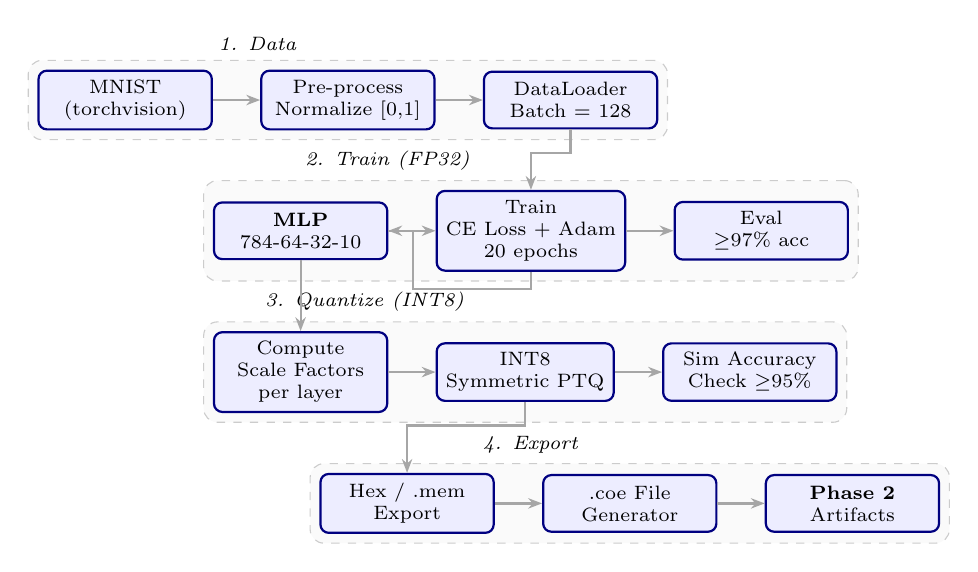
\begin{tikzpicture}[
    bl/.style={rectangle, draw=blue!50!black, thick, fill=blue!7, rounded corners=3pt,
               align=center, font=\scriptsize, minimum height=0.72cm, minimum width=2.2cm},
    grp/.style={draw=gray!40, dashed, rounded corners=5pt, fill=gray!4},
    nar/.style={-{Stealth[length=5pt]}, thick, color=gray!70},
]

% Stage 1: Data
\node[bl] (ds)  {MNIST\\(torchvision)};
\node[bl, right=0.6cm of ds] (pp) {Pre-process\\Normalize [0,1]};
\node[bl, right=0.6cm of pp] (dl) {DataLoader\\Batch = 128};

% Stage 2: Train
\node[bl, below=0.9cm of pp, xshift=-0.6cm] (mlp) {\textbf{MLP}\\784-64-32-10};
\node[bl, right=0.6cm of mlp] (tr) {Train\\CE Loss + Adam\\20 epochs};
\node[bl, right=0.6cm of tr]  (ev) {Eval\\$\geq$97\% acc};

% Stage 3: Quantize
\node[bl, below=0.9cm of mlp] (sf)  {Compute\\Scale Factors\\per layer};
\node[bl, right=0.6cm of sf]  (q8)  {INT8\\Symmetric PTQ};
\node[bl, right=0.6cm of q8]  (qv)  {Sim Accuracy\\Check $\geq$95\%};

% Stage 4: Export
\node[bl, below=0.9cm of q8, xshift=-1.5cm] (hex) {Hex / .mem\\Export};
\node[bl, right=0.6cm of hex] (coe) {.coe File\\Generator};
\node[bl, right=0.6cm of coe] (out) {\textbf{Phase 2}\\Artifacts};

% Arrows stage 1
\draw[nar] (ds) -- (pp);
\draw[nar] (pp) -- (dl);
\draw[nar] (dl.south) -- ++(0,-0.3) -| (tr.north);

% Arrows stage 2
\draw[nar] (mlp) -- (tr);
\draw[nar] (tr) -- (ev);
\draw[nar] (mlp.south) -- (sf.north);
\draw[nar] (tr.south) -- ++(0,-0.22) -- ++(-1.5,0) |- (mlp.east);

% Arrows stage 3
\draw[nar] (sf) -- (q8);
\draw[nar] (q8) -- (qv);

% Arrows stage 4
\draw[nar] (q8.south) -- ++(0,-0.3) -| (hex.north);
\draw[nar] (hex) -- (coe);
\draw[nar] (coe) -- (out);

% Group boxes
\begin{scope}[on background layer]
    \node[grp, fit=(ds)(pp)(dl),   label=above left:{\scriptsize\textit{1. Data}}] {};
    \node[grp, fit=(mlp)(tr)(ev),  label=above left:{\scriptsize\textit{2. Train (FP32)}}] {};
    \node[grp, fit=(sf)(q8)(qv),   label=above left:{\scriptsize\textit{3. Quantize (INT8)}}] {};
    \node[grp, fit=(hex)(coe)(out), label=above left:{\scriptsize\textit{4. Export}}] {};
\end{scope}
\end{tikzpicture}
\caption{Phase 1 software pipeline.}
\label{fig:pipeline}
\end{figure}

% ── 2.4 Dataset and Pre-processing ────────────────────────────────────────────
\subsection{Dataset Acquisition and Pre-processing}
We will use \texttt{torchvision.datasets.MNIST} to download the standard MNIST dataset. This interface
integrates directly with PyTorch DataLoaders and avoids an extra format conversion step. Table~\ref{tab:mnist}
summarizes the dataset properties and pre-processing steps we will apply.

\begin{table}[H]
\centering
\caption{MNIST Dataset Summary}
\label{tab:mnist}
\begin{tabular}{ll}
\toprule
\textbf{Property} & \textbf{Value} \\
\midrule
Source                   & \texttt{torchvision.datasets.MNIST} \\
Training / Test samples  & 60,000 / 10,000 \\
Image size               & $28 \times 28$ pixels, grayscale, uint8 \\
Classes                  & 10 (digits 0--9) \\
Normalization            & Divide by 255 to float [0,1]; apply mean=0.1307, std=0.3081 \\
Flatten                  & Row-major $28\times28 \to$ 784-element vector \\
Batch size               & 128 (train, shuffle=True); full 10K for test evaluation \\
\bottomrule
\end{tabular}
\end{table}

% ── 2.5 Model Training ────────────────────────────────────────────────────────
\subsection{Model Training}

We will train the MLP in PyTorch using the following configuration:

\begin{itemize}
    \item \textbf{Loss:} \texttt{nn.CrossEntropyLoss}
    \item \textbf{Optimizer:} Adam ($\eta = 10^{-3}$)
    \item \textbf{Epochs:} 20
    \item \textbf{Regularization:} \texttt{Dropout(0.2)} after FC1 and FC2
          during training only (disabled and removed before weight export)
    \item \textbf{Target:} $\geq 97\%$ top-1 accuracy on the 10K test set
\end{itemize}

Softmax will be used in the training loss but will not be exported to hardware.
In Phase 2, the MLP Core will apply \texttt{argmax} to the raw INT32 logits to
produce the predicted class. This avoids the need for \texttt{exp()} and division
in hardware.

% ── 2.6 Quantization ──────────────────────────────────────────────────────────
\subsection{Quantization}

After training, we will apply symmetric post-training quantization (PTQ) to convert
all weights from FP32 to INT8. We will use symmetric quantization (zero-point = 0)
so that the Phase 2 MAC unit does not need a zero-point subtraction in its inner loop.

\textbf{Quantization formula (per layer):}
\[
S_W = \frac{\max(|W_{\min}|,\,|W_{\max}|)}{127}, \qquad
W_q = \operatorname{clamp}\!\left(\operatorname{round}\!\left(\frac{W}{S_W}\right),\,-128,\,127\right)
\]

One scale factor $S_W$ will be saved per layer in \texttt{scales.txt} for use by
the PS during result interpretation.

If quantized accuracy drops below 94\%, we will apply quantization-aware
training (QAT) before export.

The expected Phase 1 result is a floating-point model with at least 97\% test accuracy and a quantized INT8 model with at least 95\% accuracy. A small drop after quantization is acceptable, as it allows the model to fit within the hardware constraints of the Zybo Z7-10. We will verify both results on the full 10,000-image MNIST test set before handing off to Phase 2.

% ── 2.7 Weight Export ─────────────────────────────────────────────────────────
\subsection{Weight Export}

The following files will be generated at the end of Phase 1 and handed off to
Phase 2 for Vivado BRAM initialization:

\begin{table}[H]
\centering
\caption{Phase 1 Output Files}
\begin{tabular}{llr}
\toprule
\textbf{File} & \textbf{Contents} & \textbf{Size} \\
\midrule
\texttt{W1.coe} & INT8 weights, FC1 ($784\times64$), row-major & $\approx$49\,KB \\
\texttt{W2.coe} & INT8 weights, FC2 ($64\times32$), row-major  & $\approx$2\,KB  \\
\texttt{W3.coe} & INT8 weights, FC3 ($32\times10$), row-major  & 320\,B          \\
\texttt{b1--b3.coe} & INT32 biases (64, 32, 10 values)         & 424\,B          \\
\texttt{scales.txt} & FP32 scale factor per layer              & 3 lines         \\
\bottomrule
\end{tabular}
\end{table}

All \texttt{.coe} files use the Xilinx Block Memory Generator format:
\begin{center}\small\ttfamily
memory\_initialization\_radix=16;\\
memory\_initialization\_vector=7F, 3A, FF, 80, \ldots ;
\end{center}

\texttt{scales.txt} is read by the PS (ARM Cortex-A9) for optional
dequantization of output logits. The PL does not read it directly.


\section{Phase 2: Hardware Implementation}

In Phase 2, the quantized MLP will be implemented as a hardware accelerator in the Programmable Logic (PL) of the Zynq-7010. The Processing System (PS) will provide control and communication, while the custom MLP Core in the PL will perform inference.

\subsection{IP Cores Used}

The Phase 2 hardware design will use a small set of standard Vivado IP cores together with a custom RTL MLP Core to implement the neural network accelerator.
Table~\ref{tab:ip_cores} lists the main blocks and their roles.

\begin{table}[H]
\centering
\caption{Vivado IP Cores and Their Roles}
\label{tab:ip_cores}
\begin{tabular}{lp{9cm}}
\toprule
\textbf{IP Core} & \textbf{Role} \\
\midrule
ZYNQ7 Processing System  & ARM Cortex-A9; DDR controller, UART, AXI4-Lite master ports \\
AXI Interconnect         & Routes AXI transactions between PS and PL peripherals \\
AXI GPIO                 & Control/status registers (start, done, predicted class) \\
Block Memory Generator   & BRAM initialized with Phase 1 \texttt{.coe} weight files \\
Processor System Reset   & Synchronized reset for all PL logic \\
Custom RTL: MLP Core     & Neural network datapath with AXI4-Lite slave input buffer \\
\bottomrule
\end{tabular}
\end{table}

% ── 3.2 System-Level Data Flow ────────────────────────────────────────────────
\subsection{System-Level Data Flow}

In Phase 2, test images will be stored as a byte array in DDR memory. To run inference, the ARM CPU will read one 784-byte image from DDR and write the pixel bytes into the MLP Core
input buffer over AXI4-Lite. It will then assert the start signal via AXI GPIO. The FSM inside the MLP Core will take over, reading quantized weights from BRAM and feeding them into
the MAC datapath along with the input pixels. Once inference is complete, the FSM will assert the done signal, and the CPU will read back the predicted digit.

\begin{figure}[H]
\centering
\resizebox{\textwidth}{!}{%
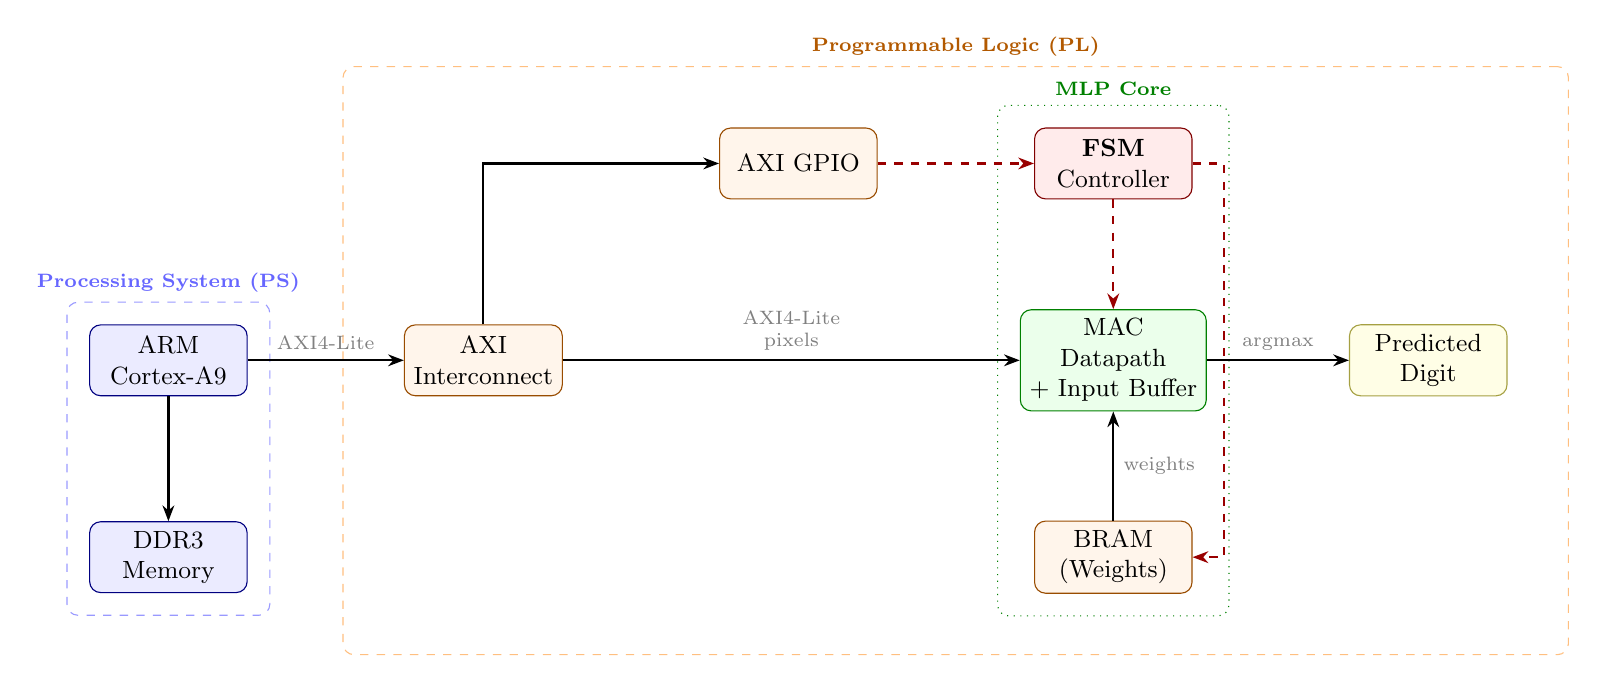
\begin{tikzpicture}[
    block/.style={draw, rounded corners, minimum width=2.0cm, minimum height=0.9cm,
                  align=center, font=\small},
    psblock/.style={block,  fill=blue!8,   draw=blue!50!black},
    plblock/.style={block,  fill=orange!8, draw=orange!60!black},
    fsmblock/.style={block, fill=red!8,    draw=red!50!black},
    macblock/.style={block, fill=green!8,  draw=green!50!black},
    arrow/.style={-{Stealth[length=2mm]}, thick},
    ctrlarrow/.style={-{Stealth[length=2mm]}, thick, dashed, draw=red!60!black},
    lbl/.style={font=\scriptsize, text=gray, align=center},
]

% Grid layout
% x cols : 0=PS,  4=AXI,  8=GPIO,  12=FSM/MAC/BRAM,  16=Result
% y rows : 0=DDR/BRAM,  2.5=main,  5=GPIO/FSM

\node[psblock]  at (0,   2.5) (ps)   {ARM\\Cortex-A9};
\node[psblock]  at (0,   0)   (ddr)  {DDR3\\Memory};
\node[plblock]  at (4,   2.5) (axi)  {AXI\\Interconnect};
\node[plblock]  at (8,   5)   (gpio) {AXI GPIO};
\node[fsmblock] at (12,  5)   (fsm)  {\textbf{FSM}\\Controller};
\node[macblock] at (12,  2.5) (mac)  {MAC\\Datapath\\+ Input Buffer};
\node[plblock]  at (12,  0)   (bram) {BRAM\\(Weights)};
\node[block, fill=yellow!10, draw=yellow!60!black]
                at (16,  2.5) (res)  {Predicted\\Digit};

% PS arrows
\draw[arrow] (ps)  -- node[above,lbl]{AXI4-Lite} (axi);
\draw[arrow] (ps)  -- (ddr);

% AXI -> GPIO: up then right
\draw[arrow] (axi.north) |- (gpio.west);

% AXI -> MAC input buffer
\draw[arrow] (axi) -- node[above,lbl]{AXI4-Lite\\pixels} (mac);

% GPIO -> FSM: control (dashed)
\draw[ctrlarrow] (gpio) -- (fsm);

% FSM -> MAC: control (dashed)
\draw[ctrlarrow] (fsm) -- (mac);

% FSM -> BRAM: addr (dashed, L-path)
\draw[ctrlarrow] (fsm.east) -- ++(0.4,0) |- (bram.east);

% BRAM -> MAC: weights
\draw[arrow] (bram) -- node[right,lbl]{weights} (mac);

% MAC -> Result
\draw[arrow] (mac) -- node[above,lbl]{argmax} (res);

% Bounding boxes
\begin{scope}[on background layer]
    \node[draw=blue!40, dashed, rounded corners, inner sep=8pt,
          fit=(ps)(ddr),
          label={[font=\scriptsize\bfseries,text=blue!60]above:Processing System (PS)}] {};
    \node[draw=green!50!black, dotted, rounded corners, inner sep=8pt,
          fit=(fsm)(mac)(bram),
          label={[font=\scriptsize\bfseries,text=green!50!black]above:MLP Core}] {};
    \node[draw=orange!50, dashed, rounded corners, inner sep=22pt,
          fit=(axi)(gpio)(fsm)(mac)(bram)(res),
          label={[font=\scriptsize\bfseries,text=orange!70!black]above:Programmable Logic (PL)}] {};
\end{scope}
\end{tikzpicture}
}% end resizebox
\caption{System-level block diagram. The PS will write pixels to the MLP Core over AXI4-Lite, assert
the start signal through AXI GPIO, and the FSM inside the MLP Core will drive BRAM access and the MAC
datapath. After inference, the PS will read the predicted digit from the MLP Core.}
\label{fig:arch}
\end{figure}


\subsection{MLP Core Internal Datapath}

The custom MLP Core will implement the main inference computation in the PL using a sequential MAC-based datapath controlled by an FSM.

\begin{enumerate}
    \item \textbf{MAC Unit:} The datapath will use 8 parallel 8-bit$\times$8-bit multipliers with 32-bit accumulators, which we expect to map to DSP48E1 slices during synthesis.

    \item \textbf{Layer Processing:} The FSM will process one layer at a time. The estimated cycle counts are: FC1 ($784\times64$): $\lceil784/8\rceil \times 64 = 6{,}272$ cycles; FC2 ($64\times32$): $\lceil64/8\rceil \times 32 = 256$ cycles; FC3 ($32\times10$): $\lceil32/8\rceil \times 10 = 40$ cycles.

    \item \textbf{ReLU:} ReLU will be implemented as a comparison with zero and will not consume DSP resources.

    \item \textbf{Weight Storage:} Each layer will have a dedicated BRAM block initialized from the Phase 1 \texttt{.coe} files. The FSM will address each BRAM sequentially during inference.

    \item \textbf{Argmax:} A comparator tree over the 10 output scores will produce the predicted digit index.
\end{enumerate}

% ── 3.4 Estimated Resource Utilization ────────────────────────────────────────
\subsection{Estimated Resource Utilization}

Table~\ref{tab:resource_est} gives an early estimate of the PL resources the proposed MLP accelerator will require. These values are based on the planned datapath structure: 8 parallel MAC
units, BRAM-based weight storage, and FSM control logic.
\begin{table}[H]
\centering
\caption{Estimated PL Resource Usage}
\label{tab:resource_est}
\begin{tabular}{lrrr}
\toprule
\textbf{Resource} & \textbf{Used (Est.)} & \textbf{Available} & \textbf{Utilization} \\
\midrule
LUTs        & $\sim$8,000 & 17,600 & $\sim$45\% \\
Flip-Flops  & $\sim$5,500 & 35,200 & $\sim$16\% \\
BRAM (36Kb) & $\sim$18    & 60     & $\sim$30\% \\
DSP48E1     & $\sim$8-16    & 80     & $\sim$10-20\% \\
\bottomrule
\end{tabular}
\end{table}

The actual resource usage will depend on the final RTL implementation and synthesis optimizations, but these estimates
suggest that the design should fit within the Zybo Z7-10's limits with room to spare for control logic and interfacing.
DSP and BRAM are the tightest constraints, since the MLP Core depends on parallel MAC units and on-chip weight storage.
Even so, the estimated usage stays well below the device limits, which gives us confidence that the planned architecture
is feasible on this platform.

At a 100\,MHz clock frequency, the estimated inference time is $6{,}272 + 256 + 40 = 6{,}568$ clock cycles, which corresponds
to about $65.7\,\mu$s per image. The actual end-to-end time will be slightly higher because the PS must also transfer the input
image and read back the result.

\section{Conclusion}

This project proposes a hardware accelerator for handwritten digit recognition on the Zybo Z7-10 using a quantized Multi-Layer
Perceptron (MLP). In Phase 1, we will train and quantize the MLP in software. In Phase 2, we will implement the quantized model
as a custom RTL accelerator in the programmable logic of the Zynq-7010.

The proposed design is intentionally kept small to fit within the LUT, DSP, and BRAM limits of the Zybo Z7-10. By combining a simple
MLP architecture with 8-bit quantization and a MAC-based datapath, we aim to demonstrate that handwritten digit inference can be
implemented on this resource-constrained platform.

Because the Phase 2 accelerator will implement the same quantized model produced in Phase 1, we expect the hardware classification
accuracy to remain close to the software accuracy, with a target of at least 95\% on the MNIST test set. The expected outcome is a
working end-to-end system where the PS transfers input images and reads back the predicted digit, while the custom MLP Core in the
PL carries out the inference.
\end{document}
